%!TEX root = main.tex
\section{Towards Dataset Understanding\label{sec:understanding}}
\par One of the key goals of visual data exploration is to promote a better understanding of the dataset to enable users to make actionable decisions. While our focus in the previous sections have focussed on intention-driven queries, where users have some knowleldge of what types of questions he may be interested in. This section discusses systems that helps users become more aware of their dataset and visualize where they are in their analysis workflow. %general query-free recommendations and continual provenance
\par Situations where there is an absence of explicit signals from the user can happen when a user is at the beginning of their analysis (commonly known as the `cold-start' problem) or when the user doesn't know what to query for, which is the finding derived from our \zv study, described in Section~\ref{sec:hypothesis}. In this section, we will describe \sbd, a system that provides data summaries and guides users through informative subsets of data, as an example of a system that promotes distribution awareness in a query-free scenario. Then, we will discuss two other types of data understanding during dynamic visual data exploration to highlight the challenges and opportunities ahead in this space.
\subsection{\sbd: Promoting Distribution Awareness of Data Subsets with Summary of Visualizations}
%Through Guided ExplorationNavigating Through
%understanding distributions (distribution awareness)
%introduce problem + challenge
\par Common analytics tasks, such as causal inference, feature selection, and outlier detection requires studying the distributions or patterns at different levels of data granularity~\cite{Anand2015,Wu2013,Heer2012}. However, it is often hard to know \textit{what} subset of data contains an insightful distribution to examine. In order to explore different data subsets, a user would first have to construct a large number of visualizations corresponding to all possible data subsets, and then navigate through this large space of visualizations to draw meaningful insights. The lack of a systematic way to perform these excercises makes the process of manually exploring distributions from all possible data subsets tedious and inefficient~\cite{Sarawagi1998,Sarawagi2000}.
%there is no systematic way to perform these exercises.
% explain what storyboard does
\par To this end, we present \sbd, an interactive visualization summarization system that automatically selects a set of visualizations to summarize the distributions within a dataset in an informative manner. Figure~\ref{sbd} illustrates an example dashboard generated by \sbd from the Police Stop Dataset \cite{police}, which contains records of police stops that resulted in a warning, ticket, or an arrest. The attributes in the dataset include driver gender, age, race, and the stop time of day, whether a search was conducted, and whether contraband was found. We requested \sbd to generate a dashboard of 9 bar chart visualizations with x-axis as the stop outcome (whether the police stop resulted in a ticket, warning, or arrest/summons) and y-axis as the percentage of police stops that led to this outcome. First, at the top of our dashboard, \sbd highlights three key data subsets that results in a high arrest rate, which looks very different trend than the overall (where the majority of stops results in tickets). Following along the leftmost branch, we learn that even though in general when a search is conducted, the arrest rate is almost as high as ticketing rate, when we look at the asian population, whether a search is conducted had less influence on the arrest rate and the trend resembles more like the overall distribution.
\begin{figure}[h!]
\centering
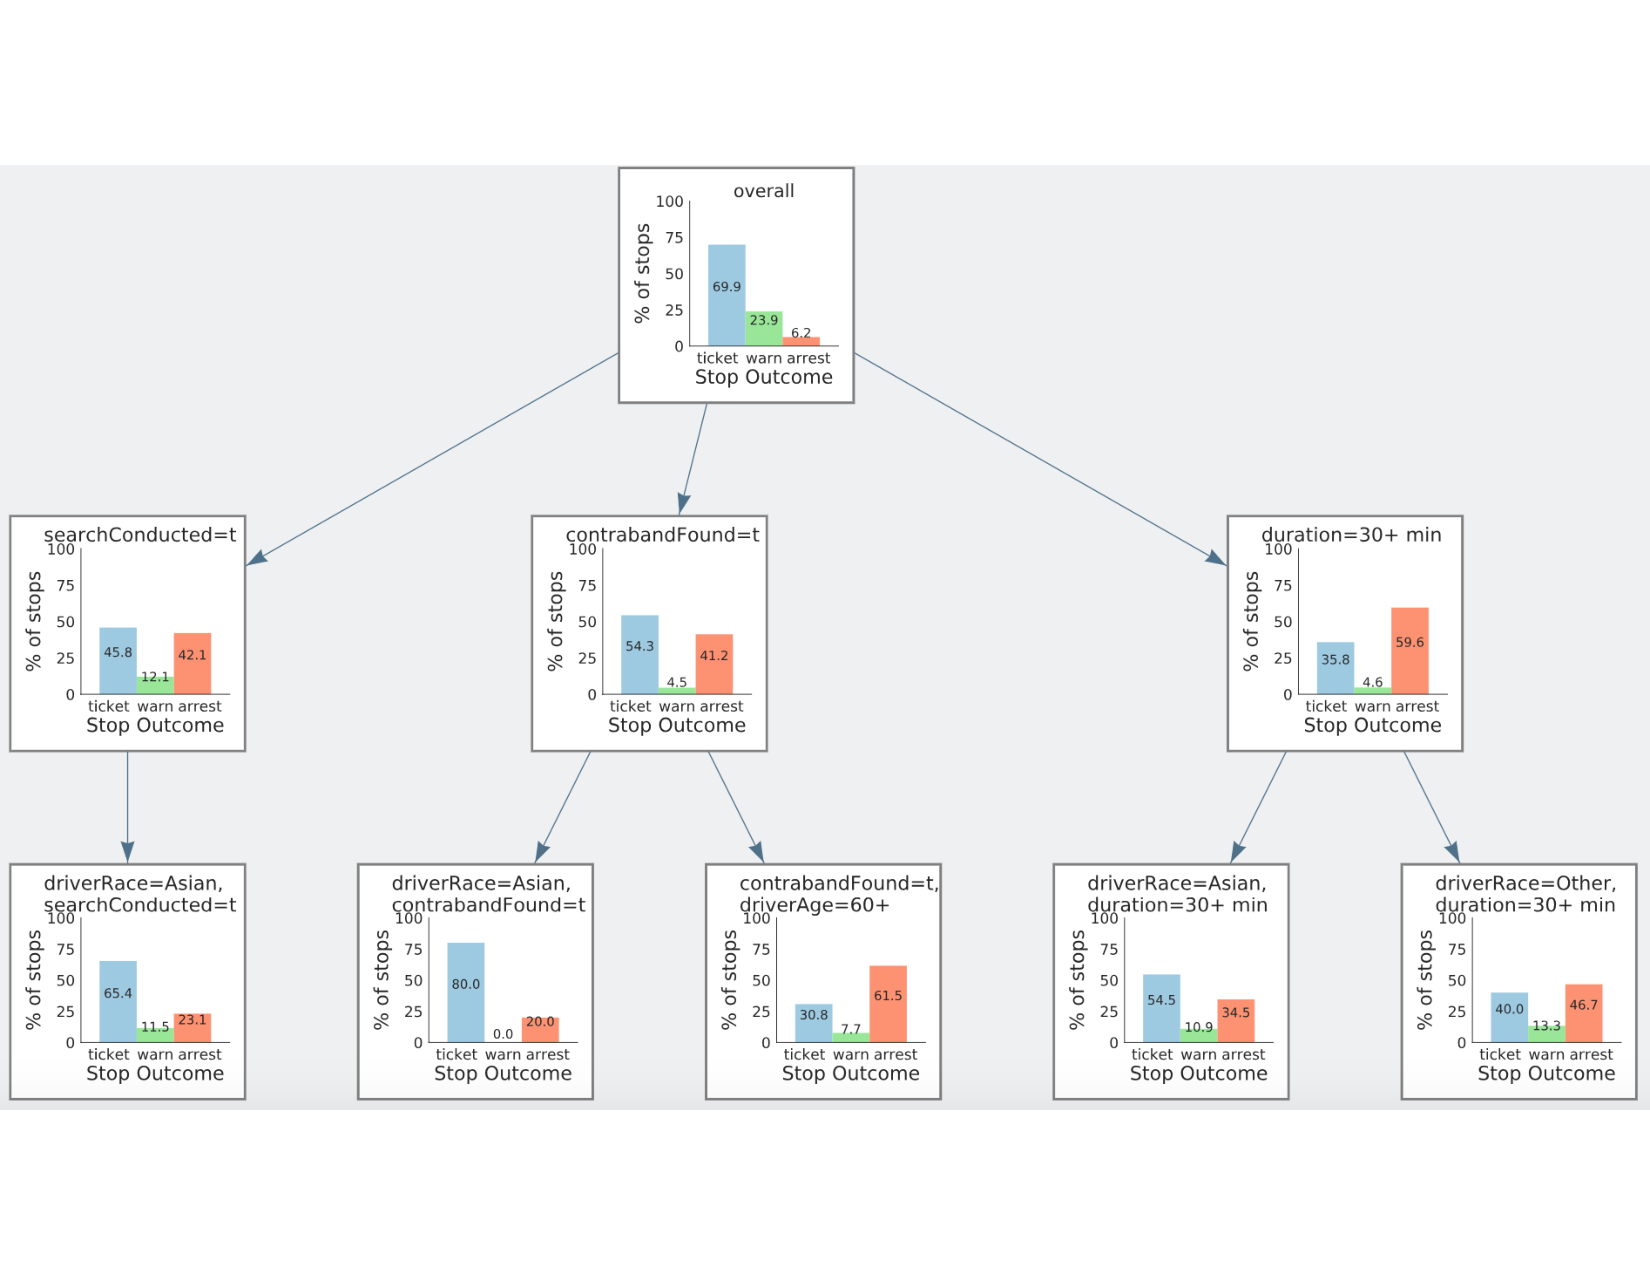
\includegraphics[width=0.7\linewidth]{figures/storyboard.pdf}
\caption{Example dashboard generated by \sbd summarizing the key insights in the Police dataset.}
\label{fig:sbd}
\end{figure} 
% one paragraph on motivation on objectives and explain lattice + traversal 
\par While such summary dashboards are useful for making sense of relationships between data subsets, finding effective visualizations to summarize a dataset is not as trivial as picking individual visualizations that maximizes some statistical measure, such as deviation~\cite{Vartak2015}, coverage~\cite{Sarvghad2017}, or significance testing~\cite{Anand2015}, which can often result in misleading summarizations. The key idea behind our work is how users formulate their expectations regarding an unseen visualization in a \textit{data subset lattice}. We make use of the idea of a data subset lattice from data cube literature to organize the relationships between different visualization. A visualization is a \textit{parent} of another visualization if the latter visualization can be derived from the first visualization by adding one additional filter constraint. 
\par Our formative user study showed that people naturally form their expectations based on one or more observed parents and that seeing a parent that well describes the unseen visualization leads participants to better estimate the unseen visualization. More importantly, in the absence of an informative parent or in the presence of multiple parents, participants can be misled to form an inaccurate expectation that exhibit higher variance. 
\par Given these insights, the goal of our system is to select \textit{interestingness} and \textit{informativeness} visualizations that can help them make more accurate predictions regarding the unseen visualizations. To model the informativeness of an observed parent in the context of an unseen visualization, we characterize the capability of the parent in predicting the unseen visualization. Our study shows that a visualization is \emph{informative} if its data distribution closely follows the data distribution of the unseen child visualization, since the visualization helps the analyst form an accurate mental picture of what to expect from the unseen visualization. While informative parents contribute to the prediction of an unseen visualization, the most interesting visualizations to recommend are those for which \emph{even the informative parents fail to accurately predict or explain the visualization}. %To model the interestingness of an unseen visualization in the context of an observed parent, we characterize the deviation between their data distributions using a distance function. The unseen visualizations whose data distributions deviate from the observed informative parents are \emph{interesting}. 
Detailed treatments of our metrics and algorithms can be found in our technical report. \dor{(CITE PLACEHOLDER) Can we put a version of the \sbd paper on arxiv so that we can cite it?}
%explain distribution awareness + its application, its relationship with dataset understnading + how it can be used in other contexts.
\par The effectiveness of \sbd largely comes from how it helps analysts become more distributionally aware of the dataset. We define \emph{distribution awareness} as the aspect of data understanding in which analysts make sense of the key distributions across different data subsets and their relationship in the context of the dataset. So that even though it may be infeasible to examine all possible data subsets, with distribution awareness, the analyst will still be able to draw meaningful insights and establish correlations about related visualizations by generalizing their understanding to make predictions regarding the unseen visualizations. Our user study evaluations show that facillatating distribution awareness through \sbd guides users to make better predictions regarding unseen visualizations, ranking attribute importance, and retreival of interesting visualizations compared to the baselines.
%building future systems that effectively guide analysts towards more meaningful stories for further investigation.
% How ----- is underexplored 
% future research 
% building systems that ---
\subsection{From Distributional to Contextual Awareness: Challenges and Opportunities}
\par The notion of distribution awareness is useful when we are looking at user understanding at one static point in time of the analysis (e.g. during cold start). In this section, we introduce a complementary notion of data understanding called \textit{contextual awareness}, which is essential when considering the dynamic setting of visual data exploration in the context of an analytic workflow.
 %In this section, we will discuss several other types of data understanding that is essential for effective visual data exploration. Recommendation providing better understanding for overall dataset and understanding. 
\par Contextual awareness is the aspect of data understanding related to understanding the \textit{situation} (what is the information that I'm currently looking and how did it come about?) and \textit{provenance} (what have I explored in the past and where should I look next?) of the data. Situational understanding involves recognizing what data is in the current scope of analysis, including making sense of the data attributes and schema and keeping track of what filter or transformations have been applied to the displayed data. Provenance understanding is related to the user's past analysis actions on the data. As an example, an analyst may be interested in how sales price of a product changes as a function of other dimensions variables, such as geographic location, year sold, and product type. Situation information informs him that he is looking at a bar chart with x = \texttt{TYPE},y = \texttt{AVG(PRICE)}, whereas provenance information points to the fact that he should explore the geographic dimension, since he has already expored the temporal attribute \texttt{YEAR}.
\par Mechanisms that facillitate distribution awareness for users can effectively couple with contextual awareness in dynamic exploration situations to help update the user's mental model on the current data context. For example, the representative and outlier patterns in \zv provides summaries of data in context. When a dataset is filtered, the representative trends are updated accordingly. By being aware of both the context and the distributions, the users becomes distributionally aware of how the typical patterns and trends of the distributions changes in a particular context. %(i.e. I'm only looking at data filtered with ....),an overview of typical trends for the data to be queried.
\par Within a dataset, provenance is essential to help users navigate and provide users with sense of coverage and completion. The notion of adding navigational cues to guide exploration in visual information spaces was first proposed by Willet et al.\cite{Willett2007} in work on \textit{scented widgets}. Scented widgets are inspired by Pirolli and Card's theory of `scent' in foraging. The widgets adds to existing interfaces by embedding visualizations that provide informational `scents', such as histogram distributions of how popular a particular value is among users or using color to encode the size of a dataset in a dropdown menu. Recently, Sarvghad et al. \cite{Sarvghad2017} have extended the idea of scented widgets to incorporate dimension coverage information during data exploration, including which dimensions have been explored so far, in what frequency, and in which combinations. Their study show that visualizing dimension coverage leads to increased number of questions formulated, findings, and broader exploration than participants who had no access to coverage information. Interpretable and non-disruptive cues that enables users to visualization provenance history helps sustain contextual awareness and guides users towards more informative next steps in their analysis.

\par Note that while the discussion above have been focussed on how to design systems that can help facillatate these aspects of user's awareness in dataset understanding, these ideas can be generalized to principles in deisinging the types of intelligent querying systems discussed in Section~\ref{sec:vague}. An intelligent visual exploration system needs to be distributionally, contextually and situationally aware, by make use of information about the data (distribution awareness), the analytic context, and situation jointly in making timely recommendations. For example, contextual awareness can inform the system that the user's current situation (x,y, encoding, etc.), while a distributionally aware system may recommend a highly-skewed data subset as interesting, a sitational aware system may realize a variable have been explored extensively in the past and recommends it accordingly. In other words, these intelligent visual query system not only needs to facillatate these aspects of data understanding, but also need to make use of this information to make inference and recommendations in an interpretable manner that can guide analysts towards meaningful stories and insights for further investigation.

% inference and descisions intepretable.
% , rather than the system's awareness of the user's context, situation ,etc. Ideally, an intelligent system  should 
% related works have focussed on making specification easier, but not really trying to understnad user intent or what might the user want to see.
